\experiment{Dining Philophers problem using Semaphores}{11/10/2023}

\section{Aim}
Implement a program for solving Dining Philosophers problem using Semaphores.

\section{Algorithm}
\begin{enumerate}
   \item Start
   \item Declare and initialize the semaphores for the chopsticks.
   \item Create 5 threads with the 'pthread\_create' function, and pass the philosopher function as an argument along with the index of the philosopher as an argument.
   \item Within the philosopher function, wait for the left chopstick to become available by calling 'sem\_wait' on the semaphore corresponding to the left chopstick.
   \item Wait for the right chopstick to become available by calling 'sem\_wait' on the semaphore corresponding to the right chopstick.
   \item Sleep for one second to simulate eating.
   \item Release the right chopstick by calling 'sem\_post' on the semaphore corresponding to the right chopstick.
   \item Release the left chopstick by calling 'sem\_post' on the semaphore corresponding to the left chopstick.
   \item In the main function, wait for all threads to complete using the 'pthread\_join' function.
   \item Stop
\end{enumerate}

\section{C Program}
\begin{lstlisting}[label={list:c_program:queue}]
#include <stdio.h>
#include <pthread.h>
#include <semaphore.h>
#include <unistd.h>

sem_t chopsticks[5];

void *philosopher(void *n)
{
   int i = *(int *)n;

   sem_wait(&chopsticks[i]); // Wait for left chopstick
   printf("Philosopher %d picks up left chopstick\n", i);

   sem_wait(&chopsticks[(i + 1) % 5]); // Wait for right chopstick
   printf("Philosopher %d picks up right chopstick\n", i);

   printf("Philosopher %d is eating\n", i);
   sleep(1); // Simulate eating
   printf("Philosopher %d has finished eating\n", i);

   sem_post(&chopsticks[(i + 1) % 5]); // Release right chopstick
   printf("Philosopher %d puts down right chopstick\n", i);

   sem_post(&chopsticks[i]); // Release left chopstick
   printf("Philosopher %d puts down left chopstick\n", i);

   printf("Philosopher %d is thinking\n", i);

   pthread_exit(NULL);
}

int main()
{
   printf("No. of philosophers: 5\n");
   int arg[5];
   pthread_t t[5];

   for (int i = 0; i < 5; i++)
   {
       sem_init(&chopsticks[i], 0, 1); // Initialize semaphores
   }

   for (int i = 0; i < 5; i++)
   {
       arg[i] = i;
       pthread_create(&t[i], NULL, philosopher, (void *)&arg[i]); // Create threads
   }

   for (int i = 0; i < 5; i++)
   {
       pthread_join(t[i], NULL); // Wait for threads to finish
   }

   return 0;
}
\end{lstlisting}
\section{Output}
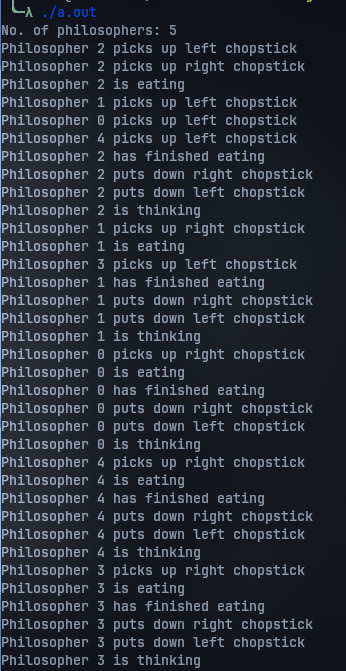
\includegraphics[width=0.5\linewidth]{Cycle_2//Outputs/philosopher.png}



\section{Result}
Successfully solved Dining Philosophers problem using Semaphores.